\setlength\abovedisplayskip{0.4pt}
\setlength\belowdisplayskip{0.4pt}

\chapter{Ultra-relativistic heavy-ion collisions}

Microseconds after the big bang, the universe was filled with a hot, dense state of strongly interacting subnuclear particles \cite{Rafelski:2013obw}. There is evidence that this phase of matter, the quark gluon plasma (QGP), is reproduced in the high energy densities reached by ultra-relativistic heavy-ion collisions \cite{Arsene:2004fa}. Measurements at the Relativistic Heavy Ion Collider (RHIC) and the Large Hadron Collider (LHC) are consistent with the QGP having the sheer viscosity of a perfect fluid \cite{Long:796947}. As such, the QGP will not obscure the initial conditions of the pre-collision heavy-ion. Therefore heavy-ion initial state properties must be rigorously measured to better distinguish between the effects of the QGP and of the inherent properties of the nucleus.

This thesis seeks to further knowledge of initial state phenomena by measuring the gluon Wigner distribution within the nucleus. In the context of coherent dijet photoproduction from ultra-peripheral collisions (UPC), the Wigner distribution of elliptic gluons is encoded in the angular correlations of the dijet transverse momentum and the proton recoil momentum \cite{Hagiwara:2016kam}. UPC have strongly suppressed hadronic activity, with all interactions between nuclei being mediated by the electromagnetic field \cite{Contreras:2015dqa}. This photo-nuclear interaction is understood via the equivalent photon approximation arising the Weizacker-Williams formalism \cite{vonWeizsacker:1934sx}\cite{Williams:1934ad}. 

A dataset of ultra-peripheral collision data was taken during the 2015 Pb-Pb run at the Compact Muon Solenoid (CMS). UPC have been shown to pass vetos on activity in the Hadronic Forward Calorimters (HF). The angular correlations of the UPC dijets are measured and used to constrain the elliptic gluon in two bins of dijet total transverse momentum. 

\section{The Standard Model}

The Standard Model describes the fundamental particles of the universe in terms of fermions and bosons. Fermions are particles with half-integer spin, while bosons have integer-spin. This difference in spin has far reaching consequences. Fermions must obey the Pauli Exclusion Principle: only one fermion at a time can occupy a given state. However, multiple bosons can simultaneously occupy a specific state \cite{Dyson:1967:SM}. Subnuclear particles -- protons and neutrons -- contain large numbers of both fermions and bosons. Fermions and bosons have different stastical properties. Fermi-Dirac stastistics describe the energy distribution of fermions. Likewise, the boson energy distribution is described by Bose-Einstein statistics \cite{Huang_1987}. 

Among the fermions are the leptons, neutrinos, and quarks. The leptons consist of the electron, muon, and tau, as well as their anti-particles. The leptons are seemingly fundamental: high energy experiments have yet to observe internal lepton-structure. Neutrinos are weakly interacting particles detected primarily through the precise measuring of missing transverse energy in the products of particle collisions. Quarks are the constituent particles of baryons, which contain three valence quarks, and mesons, which contain two valence quarks. In addition to the valence quarks are the sea quarks, which appear and disappear as quark-antiquark pairs within hadrons. The hadrons are particles made of quarks and gluons. Gluons are particles that mediate the strong nuclear force; likewise, photons mediate the electromagnetic force, and weak-gauge bosons mediate the weak nuclear force. A fourth boson, the graviton, is expected to transmit the gravitational force, but this particles existence has not been verified \cite{Halzen:1984mc}. 

The behavior of fundamental particles is best described within the framework of quantum field theory (QTF). QFT defines a Lagrangian for fundamental particles. This Lagrangian then predicts the outcome of particle collisions. Different terms in the Lagrangian correspond to the various interactions between particles. The Standard Model Lagrangian, $\mathcal{L}_{Standard Model}$ can be broken down into three basic terms:	
\begin{equation}
\mathcal{L}_{Standard Model} = \mathcal{L}_{QED} + \mathcal{L}_{QCD} + \mathcal{L}_{Higgs} + ... ,  
\end{equation} 
Where $\mathcal{L}_{QED}$ is the QED Lagrangin, $\mathcal{L}_{QCD}$ is the QCD Lagrangian, and $\mathcal{L}_{Higgs}$ is the Higgs Lagrangian. The QED and QCD Lagrangians will be the most important in what follows \cite{Halzen:1984mc}. 

The most accessible approach to quantum field theory is through the use of Feynman diagrams. First, one imagines an interaction between particles. Then, one draws this process into a Feynman diagram, which is essentially a pictorial representation of exchanges between particles. The Lagrangian can be interpreted into Feynman rules. These rules describe how the Feynman diagram translates into a calcuation for the quantum mechanical amplitude of the process. The quantum mechanical amplitude, in turn, is proportional to the cross-section of the process. This is important because, sense the cross-section is invariant between experiments, one can use it to effectively test for invariant quantities in the Lagrangian \cite{Peskin:1995ev}.

\section{Quantum electrodynamics}

In classical electrodynamics, all of electrical and magnetic phenomena can be derived from four fundamental equations: Maxwell's laws. Below these equations are given in their differential form. 

Gauss's law relates the divergence of a static electric field, $\vec{E}$, to it's source charge density, $\rho$,
\begin{equation}
\triangledown\cdot\vec{E}= \frac{\rho}{\epsilon_o},
\end{equation}
where $\epsilon_o$ is permittivity of free space. Gauss's law for a static magnetic field, $\vec{B}$, reveals the stark contrast between electricity and magnetism. The diverence of a static magnetic field is always a net 0. This reflects the seeming non-existence of magnetic monopoles.  
\begin{equation}
\triangledown\cdot\vec{B}=0
\end{equation}
Faraday's law describes the curl of an electric field in terms of the dynamics of a magnetic field. The electric field and the magnetic field are coupled, and a change in one will affect the properties of the other. For a given electric field, $\vec{E}$, the curl is equal to the partial derivative of a magnetic field, $\vec{B}$, with respect to time, $t$,
\begin{equation}
\triangledown\times\vec{E}=-\frac{\partial\vec{B}}{\partial t}.
\end{equation}
Ampere's law addresses the curl of a magnetic field, $\vec{B}$, and once more the absence of magnetic monopoles gives rise to distinct properties. In addition to the partial derivative of $\vec{E}$ with respect to time $t$, there is a corrective term for the electric charge current density, $\vec{J}$, and the sum is multiplied by $\mu_o$, the permeability of free space,
\begin{equation}
\triangledown \times \vec{B} = \mu_o \left(  \vec{J} + \epsilon _{o} \frac{\partial \vec{E}}{\partial t} \right ).
\end{equation}
The complementarity of the classical electric and magnetic fields gives rise to the photon flux so important for ultra-peripheral collisions, and will be discussed in greater detail in the next chapter \cite{griffiths1999introduction}.

Quantum electrodynamics (QED) is a theory of electromagnetic interaction in terms of relativistic quantum field theory. The QED Lagrangian is given below,
\begin{equation}
{\mathcal {L}}={\bar {\psi }}(i\gamma ^{\mu }D_{\mu }-m)\psi -{\frac {1}{4}}F_{\mu \nu }F^{\mu \nu },
\end{equation} 
where $\psi$ is spin-$\frac{1}{2}$ field, $\gamma^\mu$ are the Dirac matrices, $D_\mu$ is the gauge covariant derivative, $m$ is the electron mass, and $F_{\mu\upsilon}$ is the electromagnetic field tensor \cite{Peskin:1995ev}.

QED addresses three specific processes: photon motion, electron motion, and the emission, or absorption, of a photon by an electron. To do this, first a Lagrangian is established based on Maxwell's laws and quantum mechanics. The photon constitutes a spin-1 solution to the differential equations derived from the QED Lagrangian. Likewise, electrons are described, at non-relativistic scales, by the Schrodinger equation, at relativistic scales by the Dirac equation. Figure \ref{fig:qedFeynman} shows the resulting processes allowed by QED: the translation of an electron, the translation of a photon, and the scattering of a photon off an electron \cite{Griffiths:2008zz}. 

\begin{figure}[h!]
\begin{centering}
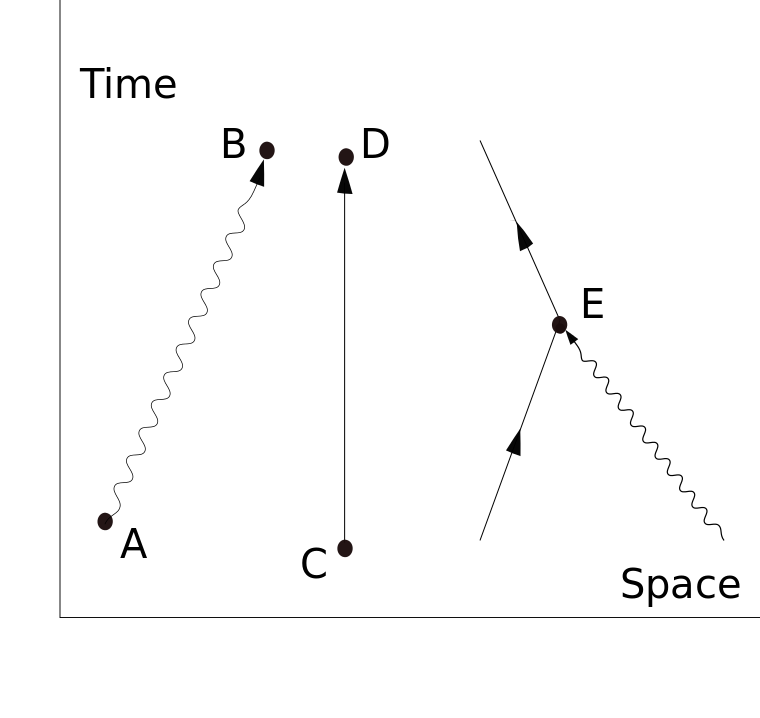
\includegraphics[width=4in]{Chapter1/importfigs/Feynman_Diagram_Components.png}
\par\end{centering}
\caption{QED Components of Feynman Diagrams (Plot from WikiCommons). \label{fig:qedFeynman}}
\end{figure}

The QED coupling constant, $\alpha_{QED}$, is approximately ~1/137 at perturbative scales \cite{Bouchendira:2010es}. In general, the cross section of a given process is proportional to the $(\alpha_{QED})^n$ where $n$ is the number of vertices in the Feynman diagram. The more complex the Feynman diagram, the smaller it's cross section. However, at small scales, i.e. non-perturbative momentum transfers $Q^2$, the coupling constant increases:
\begin{equation}
\alpha_{QED}(Q^2) = \frac{ \alpha_{em}}{(1 - \frac{\alpha_{em}}{3\pi})\mathrm{ln}(\frac{Q^2}{m^2}) },
\end{equation}
where $\alpha_{QED}(Q^2)$ is the QED coupling constant at high $Q^2$, $\alpha_{em}$, and $m$ is the electron mass \cite{Abbiendi:2005rx}. High values of $Q^2$ are non-perturbative because, at small scales and high momentum, the fluctuation of photons into electron-positron pairs begins to saturate. Particle and anti-particle pairs can pop into exist, persist a short time, and then annihilate so long as quantum numbers are conserved. 

\section{Quantum chromodynamics}

The quarks are a family of fermions that compose the baryons and the mesons. Baryons consist of three quarks in a color neutral state, while mesons consist two quarks in a color neutral state. "Color" in this context refers to the six kinds of strongly-interacting charge available to quarks: red and anti-red, blue and anti-blue, and green and anti-green. Color charge has no relation to optical phenomena, but provides a useful analogy for the stable combinations of quarks. The net color-charge of a baryon or meson is colorless. By way of analogy, a red quark, green quark, and blue quark can together form a hadron, in the way that conventional red, green, and blue can together form white \cite{Brock:1993sz}. 

Gluons are the QCD analogues of the photons in QED. Gluons are spin-1 and massless, but unlike photons, which do not carry electromagnetic charge, gluons carry strongly-interacting charge: color. Color comes six varieties: red, antired, blue, antiblue, green, and antigreen \cite{Wilczek:2000ih}. The QCD Lagrangian, which encodes the interactions of gluons and quarks, is given below,
\begin{equation}
{\mathcal {L}}_{\mathrm {QCD} }={\bar {\psi }}_{i}\left(i(\gamma ^{\mu }D_{\mu })_{ij}-m\,\delta _{ij}\right)\psi _{j}-{\frac {1}{4}}G_{\mu \nu }^{a}G_{a}^{\mu \nu },
\end{equation}
where $m$ now represents the quark mass, the $\delta_{ij}$ is the delta function and $G_{\mu \nu }^{a}$ is gluon field tensor,  
\begin{equation}
\displaystyle G_{\mu \nu }^{a}=\partial _{\mu }{\mathcal {A}}_{\nu }^{a}-\partial _{\nu }{\mathcal {A}}_{\mu }^{a}+gf^{abc}{\mathcal {A}}_{\mu }^{b}{\mathcal {A}}_{\nu }^{c}.
\end{equation}
The SU(3) group of the quarks is indexed as $i,j,...$; the adjoint SU(3) group, for the gluons, is indexed $a,b,c$. ${\mathcal {A}}_{\nu }^{a}$ is the gluon field, $f^{abc}$ are the SU(3) structure constants, and $g$ is the strong coupling \cite{Schafer:2005ff}. 

Unlike QED, the QCD coupling increases with distance \cite{Bethke:2006ac}. Figure \ref{fig:runningQCDCoupling} shows the running of the QCD coupling with $Q^2$:
\begin{equation}
\alpha_{QCD}(Q^2) = \frac{4 \pi }{(11 - \frac{2}{3}n_f)\mathrm{ln}(\frac{Q^2}{\Lambda^2_{QCD}}) } ,
\end{equation}
where $n_f$ is the number of quark flavors, $Q^2$ is the momentum transfer, and  $\Lambda^2_{QCD}$ is the mass scale \cite{Deur:2016tte}. The running coupling has the practical consequence of the strong-interactions being stronger in high momentum transfer collisions. The direct results of the running QCD coupling include the dual phenomena of asymptotic freedom and color confinement. At large distances, string tension describes the binding force of the quarks. At short distances, however, Coulomb-like interactions dominate \cite{Bjorken:1968dy}. The QCD coupling constant can be measured via the cross-section of inelastic proton-proton collisions, and also the cross section of electron-positrons into triple jets \cite{Thomson:2013zua}. 
\begin{figure}[h!]
\begin{centering}
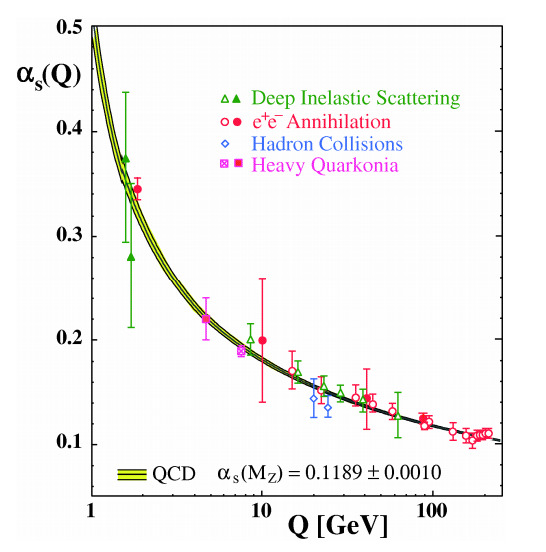
\includegraphics[width=4in]{Chapter1/importfigs/qcd_coupling_bethke.png}
\par\end{centering}
\caption{QCD Coupling Constant vs. $Q^2$ \cite{Bethke:2006ac} \label{fig:runningQCDCoupling}}
\end{figure}

Within the nucleus, a proton can be thought of as a bubble in a vacuum. Debrye screening exerts a pressure on the proton. This pressure is responsible for the size of the proton \cite{CGC2Lec}\cite{CGCandGlasma}.

\section{Deep inelastic scattering}

At the turn of the century, Ernst Rutherford probed the gold atom by bombarding a gold sheet with alpha-particles, i.e. helium nuclei. The angular distribution of the scattered alpha-particles demonstrates that the mass of the atom is concentrated in a small volume, i.e, the atom is mostly empty space. Further experiments revealed that the atomic nuclei consisted of separate positively and neutrally charged particles: protons and neutrons. Even though colliders have become more sophisticated, scattering experiments are the basic tool for exploring the nucleus. The higher the center of mass energy, the more experiments can probe the nuclear phase-space diagram.

Deep inelastic scattering commonly refers to the scattering of a leptons off hadrons. Experiments at HERA focused on electron-proton collisions. In these collisions, the electron was used as a source of photons and neutrinos. When these particles scatter off the proton, the dependence of the collision cross section, on momentum transfer and scattering angle of the source electron, reflects the structure of the proton. These experiments provided the first evidence of two phenomena: the parton model and Bjorken-scaling. 

Momentum transferred, expressed as $Q^2$, is an important quantity for characterizing DIS measurements. In addition to $Q^2$, Bjorken-x is necessary to describe the nuclear phase space. Bjorken-x represents the momentum fraction of partons. In the context of lepton-proton scattering, it was observed that in high momentum transfers limit the structure functions of the proton were functions of $Q^2/\upsilon$, where $Q^2$ is the squared four-momentum of the virtual photon emitted by the electron, and $\upsilon$ is the energy lost by the electron in the collision \cite{Bjorken:1968dy}. 

The parton model, first proposed by Richard Feynman, posits that hadrons in general, and nucleons in specific, are made of more fundamental constituent particles which may or may not be the quarks implied by the SU(3) symmetry. In addition to the quarks, the partons also include any field quanta associated with nuclear forces. In time, these field quanta are dubbed "gluons".

"Scaling" is an interpretation of the data from deep inelastic scattering (DIS). First proposed by James Bjorken, scaling is reflected in the incoherence of photon-proton interactions at photon energies above 1 $GeV/c$ \cite{Bjorken:1982qr}. Predictions from perturbative QCD are in good agreement with DIS data from HERA, as seen in figure \ref{fig:qcdBjorkenX} \cite{Shimizu:2009fc}. In this graph the Bjorken-x momentum fraction is designated $x$, and $\sigma_r$ represents the $F_2$ structure function, and $Q^2$ is the transferred momentum from the electron to the proton. The order of magnitude of $\sigma_r$ set by the Bjorken-x.

\begin{figure}[h!]
\begin{centering}
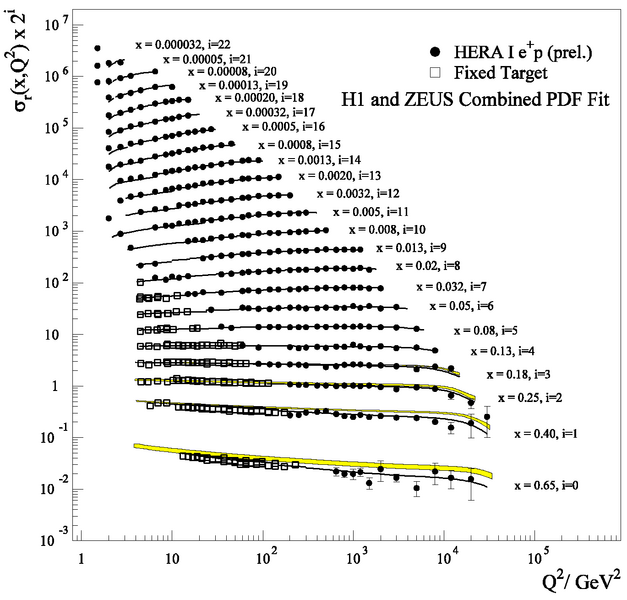
\includegraphics[width=4in]{Chapter1/importfigs/scholarpedia_bjorken_x_qcdExp.png}
\par\end{centering}
\caption{Collision Cross Section vs Bjorken-x, theory and data \cite{Shimizu:2009fc} \label{fig:qcdBjorkenX}}
\end{figure}

At the small scales probed by high energy photons, the decreasing QCD coupling causes quarks and gluons to interact weakly. This phenomena is called "asymptotic freedom". Because gluons themselves carry color charge, the gluons about a quark tend to have an anti-screening behavior: the gluon color adds to the quark color, increasing the net color charge of the area. At smaller distances to a quark, then, there are fewer and fewer gluons augmenting the color interaction.

The HERA results show that the parton density rapidly increases as the momentum fraction decreases. Conservation of momentum demands that the splintering of partons must eventually cease. The specific saturation point, where recombination begins dominates, is a characteristic of the heavy-ion initial state  and could be used to recognize the onset of QGP. 

\section{Parton distribution functions}

QCD describes the interaction between quarks and gluons, but within a nucleon the calculations are too complicated to solve for the behavior of each individual parton. Theorists compromise using the factorisation theorem to use data frome DIS experiments to make predictions. The factorisation theorem is discussed in greater detail later in this theorist. Parton distribution functions (PDFs) are a method of encoding data from DIS experiments in the form of probability density. PDFs give the probability of finding a species of parton with given momentum fraction, $x$, and a given squared energy scale, $Q^2$ \cite{Martin:2009iq}\cite{Eskola:2008ca}\cite{Pumplin:2002vw}\cite{cmsJpPP}.

In electron-proton deep inelastic scattering, the electron interacts with the proton electromagnetically by the emission of a virtual photon. This virtual photon has a four momentum $q$ and a virtuality $Q^2 = - q^2$. When virtuality is low, the virtual photon is approximately "real"; these quasi-photons are discussed in greater detail in the next chapter. The virtual photon, originating from the e. lectron, interacts with a parton and changes its initial momentum fraction, $x$. The $Q^2$ of the probing virtual photon and Bjorken-x of interacting parton are determined from the collision products. The whole data sample can be used to fill out a probability density, $F_i(x, Q^2)$, of finding a parton species $i$ at a given momentum fraction $x$ with a probe of virtuality $Q^2$.

One can use the Wigner distribution to tomographically image the internal structure of the nucleus \cite{Hatta:2016dxp}. The nucleus manifests different structures at varying momentum fractions; specifically, small momentum fractions exhibit gluon saturation \cite{Boer:2011fh}; see figure \ref{fig:nuclImag} for an illustration of how the nucleus appears at varying momentum fractions.

\begin{figure}[h!]
\begin{centering}
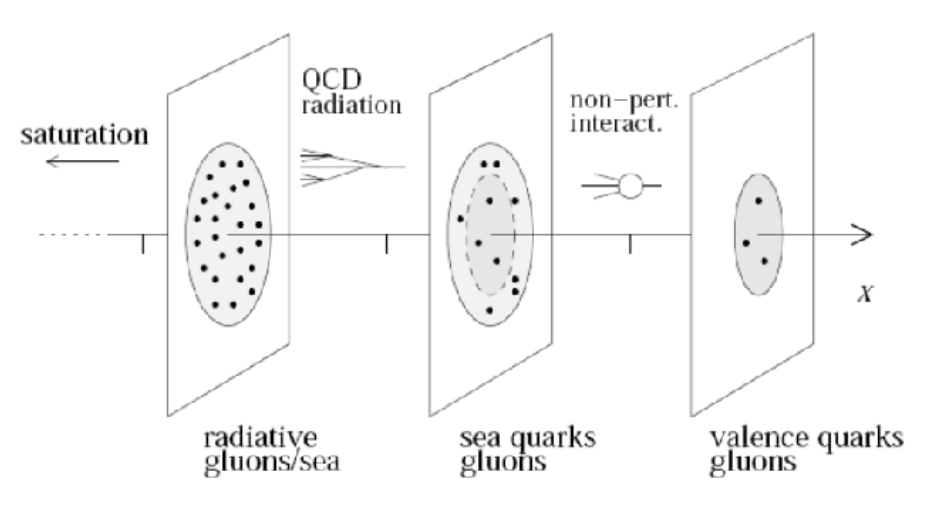
\includegraphics[width=7in]{Chapter1/importfigs/imaging_the_nucleon_upc_dijets_pres.png}
\par\end{centering}
\caption{Subnuclear tomography (Ask Daniel again) \label{fig:nuclImag}}
\end{figure}

The quantum field theory lagrangian of the strong interaction is relatively simple, but because of confinement and asymptotic freedom the hadronic bound states are too complex for an analytic solution. Furthermore, collider experiment data requires a quantitative interpretation to be useful. The gap between QCD and heavy-ion data is bridged using the parton model, which considers hadrons as composed of quarks and gluons. Parton density functions (PDFs) model the longitudinal momentum distribution of the partons. PDFs are supplemented by transverse momentum distributions (TMDs) and generalized parton distributions (GPDs). In addition to transverse momentum, GPDs describe the transverse spatial distribution. TMDs and GPDs are derived from the final state particles of a collision. Markus Diehl maps the relationship between various distribution functions in figure \ref{fig:gpdTMDWeb} \cite{Diehl:2003ny}.

\section{Evidence of quark gluon plasma}

In the 1980 - 2000, the Super Proton Synchrotron (SPS) and the Relativistic Heavy Ion Collider (RHIC) performed heavy ion experiments to study the possibility of deconfined plasma in a high parton density medium \cite{spsHI}\cite{ags2rhic}\cite{etaOvSinit}. These experiments confirmed the developing model of the QCD phase space; see figure \ref{fig:QCDPhase} \cite{Bhalerao:1695331}. Essentially, quark matter organizes itself differently depending on temperature and baryon density. At low energies, quark matter exists in bound states: the hadrons. However, in the high energy limit, quarks and gluons take the form of a strongly interacting plasma: QGP. The QGP represents the extreme case of asymptotic freedom; the QCD coupling constant becomes small enough that quarks ang gluons no longer behave as bound states. There are two ways of achieving the high energies necessary to form QGP. High baryon densities cause the quarks of separate hadrons to interact at small distances where asymptotic freedom takes effect. It is not currently possible to achive these densities in laboratory experiments, though this state is thought to occur in neutron stars. By contrast, it particle collider's like the LHC increase the energy density by colliding heavy-ions at ultra-relativistic velocities. The high temperature environment thus produced manifests QGP. The early universe, mere milliseconds after the Big Bang, is thought to have existed as QGP \cite{Hands:2001ve}.

\begin{figure}[h!]
\begin{centering}
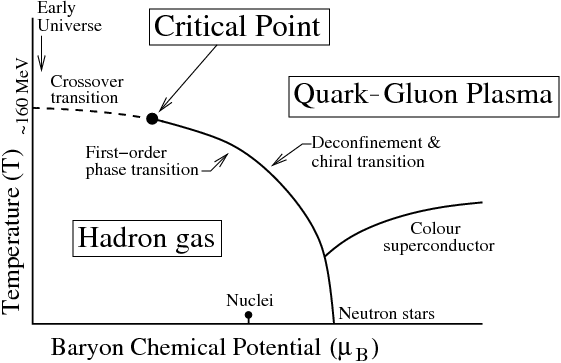
\includegraphics[width=4in]{Chapter1/importfigs/byr13.png}
\par\end{centering}
\caption{QCD Phase Diagram \cite{Bhalerao:1695331} \label{fig:QCDPhase}}
\end{figure}

There are a number of experimental signatures of QGP. Thermal physics understands phase transitions as occuring at specific temperatures and densities. At the boundary between two phases, one can define a critical point at which there is a seemingly discontinuous change in the behavior of observables. For the SPS and RHIC heavy-ion program the main observables were charm suppression and strangeness enhancement, elliptic flow, and jet quenching \cite{Gyulassy:1990ye}\cite{Matsui:1986dk}\cite{Margetis:2000sv}.

The QGP is thought to suppression the production of $J\Psi$ mesons in heavy-ion collisions. Figure \ref{fig:jpsiSupp} shows the suppression of $J/\Psi$ with respect to Drell-Yan scattering in Pb-Pb collisions at SPS \cite{spsHI}.
\begin{figure}[h!]
\begin{centering}
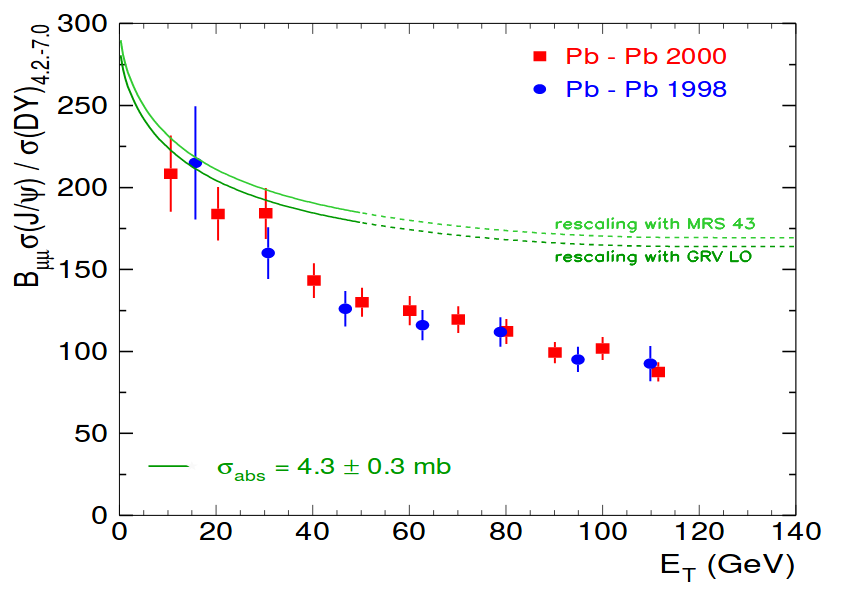
\includegraphics[width=4in]{Chapter1/importfigs/jpsiSupp.png}
\par\end{centering}
\caption{$J/\Psi$ suppression in Pb-Pb collisions \cite{spsHI} \label{fig:jpsiSupp}}
\end{figure}

The predicted viscosity of QGP would cause elliptic flow in the overlap region of heavy-ion collisions \cite{phobosFlow}. At RHIC, it was demonstrated that heavy-ion collisions can produce a medium that exhibits elliptic flow. The angular correlations of the final state particles, produced by heavy-ion collisions, were analyzed and shown to be consistent with the medium flowing as a nearly ideal fluid \cite{Chatrchyan:2013nka}. "Ideal fluid" refers to how the high temperature nuclear medium can be modelled by hydrodynamic equations in which the shear viscosity is extremely low \cite{Karsch:2000kv}. Viscosity is a measure of how readily a medium converts kinetic energy into thermal energy. For example, when highly viscous material like honey is struck with projectiles, almost all of the kinetic energy of the projectile will be converted into thermal energy within the honey, with only slight deformations, i.e. "splashes", to the honey's volume. 

In so far as the QGP is a perfect medium, the initial state properties of the heavy-ion will propagate through the collision and have a significant effect on the final state particles. The angular distribution of final state particles can be modelled using Fourier series,
\begin{equation}
 1+\sum^{\infty}_{n=1}2v_{n}\mathrm{cos}\left[n\left(\phi-\Psi\right)\right],
\end{equation}
where $n$ is the order of the Fourier expansion, $v_n$ is the Fourier coefficient, $\phi$ is the azimuthal angle, and $\Psi$ is the event-plane angle. The 2nd order term, $v_2$, is referred to as "elliptic flow" and is predicted to quantify the pressure gradient of the overlap-region in the heavy-ion collision. The over-lap region is an ellipse, with a long axis and a short axis. Figure \ref{fig:overlap} is an illustration of the overlap region of a heavy-ion collision. Because the pressure gradient is higher for the short axis than for the long axis, the nuclear medium in the overlap region will flow outward along the short axis, and this is reflected in the alignment of the tracks in the direction of the flow \cite{Abelev:2012ola}\cite{Ollitrault:1992bk}\cite{Sorensen:2009cz}\cite{Bhalerao:2003yq}\cite{Borghini:2001zr}\cite{Ackermann:2000tr}\cite{Borghini:2004ke}. 

\begin{figure}[h!]
\begin{centering}
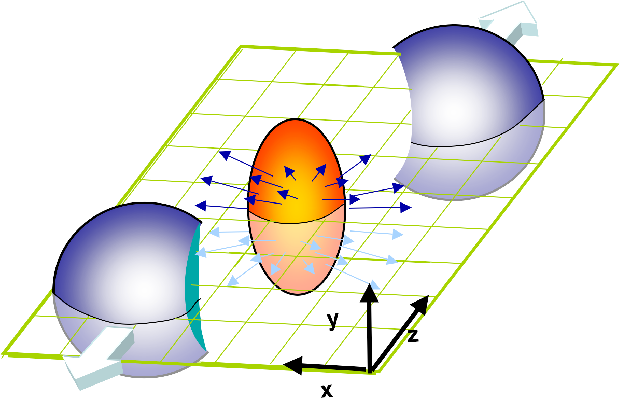
\includegraphics[width=4in]{Chapter1/importfigs/elliptic_flow_3D_medium.png}
\par\end{centering}
\caption{Heavy-ion collision overlap region \label{fig:overlap}}
\end{figure}
The viscosity of the nuclear medium directly affects how the initial properties of the overlap region affect the elliptic flow. A highly viscous medium will resist deformation such that the shape of the overlap region, i.e. its ellipticity, will not necessarily carry over to the final-state tracks. However, because the QGP medium is a nearly ideal liquid, the elliptic correlation of the final-state should arise from that of the inital-state. The RHIC result emphasizes the great importance of a precisely understood heavy-ion initial state. Figure \ref{fig:hiFlow} compares the $v_2$ elliptic flow results from various heavy-ion experiments \cite{spsHI}.
\begin{figure}[h!]
\begin{centering}
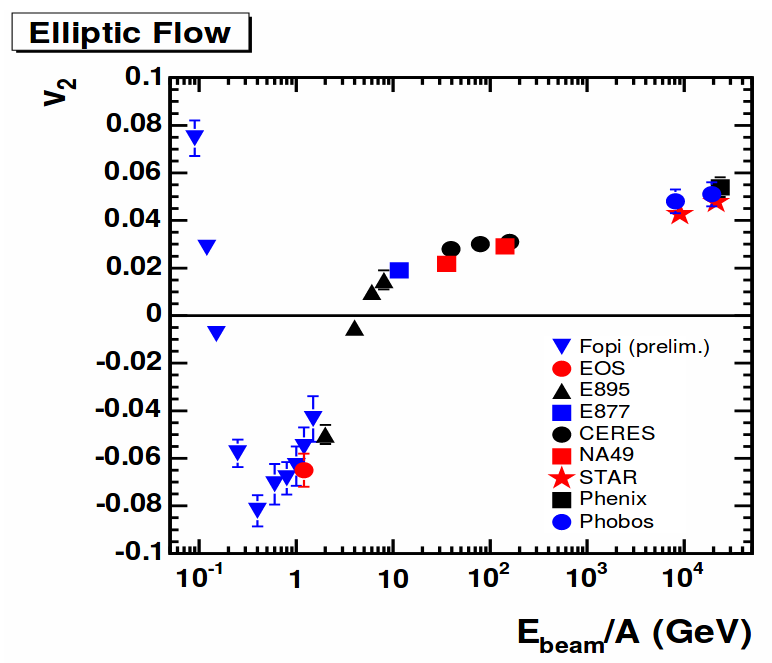
\includegraphics[width=4in]{Chapter1/importfigs/elliptic_flow.png}
\par\end{centering}
\caption{$v_2$ vs collision energy \cite{spsHI} \label{fig:hiFlow}}
\end{figure}


Figure \ref{fig:exampleStarKine} shows results from $\sqrt{S_{NN}}=130$ GeV $Au+Au$ collisions. The hydrodymanic limit is thought to describe the behavior of QGP. At lower centrality the hydrodynamic limit is in good agreement with data, but the overestimation of data at high centrality is consistent with the rapid thermalization of QGP shortly after collision. The linear $p_T$ dependence of elliptic flow implies that the expansion is enhanced in the collision plane \cite{Ackermann:200tr}. 

\begin{figure}%
    \centering
    \subfloat[label 1]{{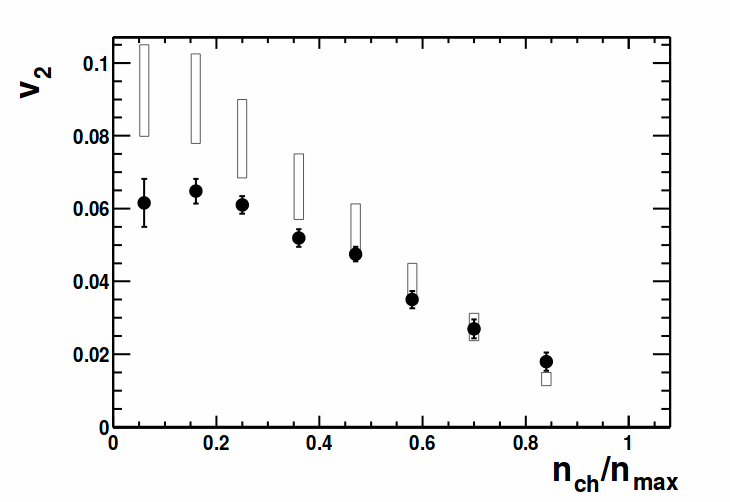
\includegraphics[width=6cm]{Chapter1/importfigs/star_130_fig3.png} }}%
    \qquad
    \subfloat[label 2]{{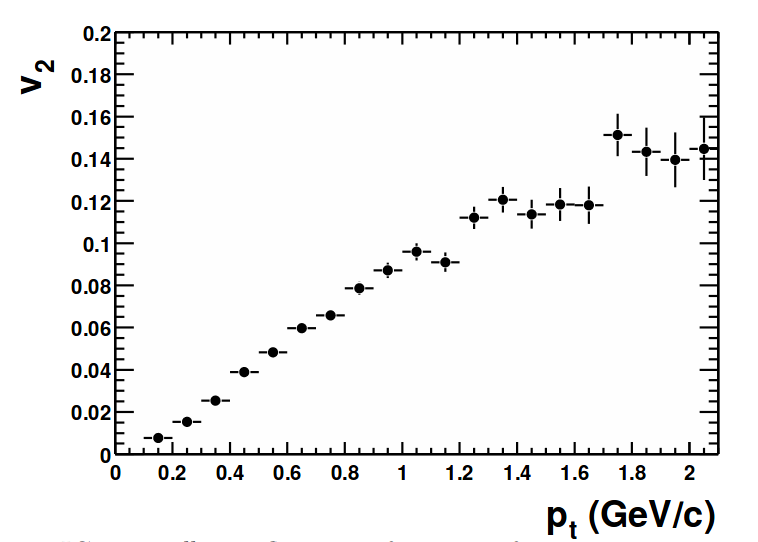
\includegraphics[width=6cm]{Chapter1/importfigs/star_130_fig4.png} }}%
    \caption{STAR $Au+Au$ at $\sqrt{s_{NN}}=130$ GeV, (left)$v_2$ vs centrality and (right)$v_2$ vs $p_T$ \cite{Ackermann:2000tr}}%
    \label{fig:exampleStarKine}%
\end{figure}

Figure \ref{fig:exampleRidge} displays one of the most striking phenomena associated with heavy-ion flow: "the Ridge". There is a distinct pattern to the two-particle correlations of high $p_T$ tracks in heavy-ion collisions. Notice that compared to pPb data the PbPb ridge is narrower, implying a stronger correlation and more pronounced elliptic flow \cite{Chatrchyan:2013nka}. 

\begin{figure}%
    \centering
    \subfloat[label 1]{{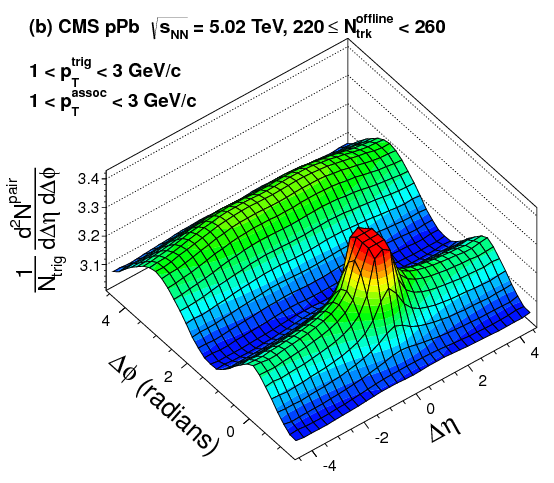
\includegraphics[width=6cm]{Chapter1/importfigs/corr2D_pPbNew_pt0-0_nmin220_nmax260_20130206.png} }}%
    \qquad
    \subfloat[label 2]{{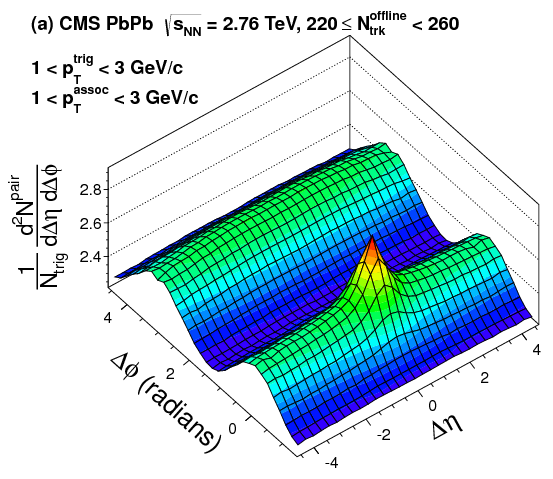
\includegraphics[width=6cm]{Chapter1/importfigs/corr2D_PbPb_pt0-0_nmin220_nmax260_20130325.png} }}%
    \caption{CMS (left) pPb and (right) PbPb, angular correlations \cite{Chatrchyan:2013nka}}%
    \label{fig:exampleRidge}%
\end{figure}

\begin{figure}[h!]
\begin{centering}
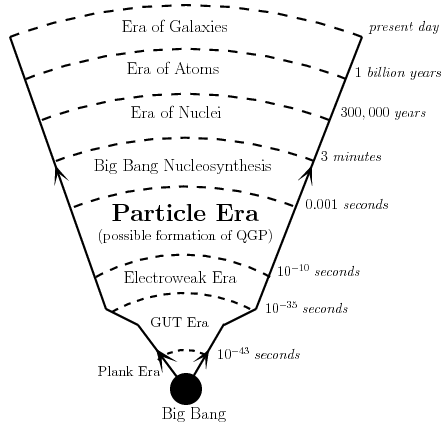
\includegraphics[width=5in]{Chapter1/importfigs/fig_bb_timeline.png}
\par\end{centering}
\caption{History of the Universe \cite{Bandyopadhyay:2017wip} \label{fig:history}}
\end{figure}

The QGP is particularly interesting because of its implications for the early universe. Figure \ref{fig:history} is a simplified cosmological timeline. In the first hundred or so microseconds after the Big Bang, the universe was small, dense, and highly energetic \cite{Bandyopadhyay:2017wip}. The energy density of the early universe would have been in excess of 1 $GeV/(fm)^3$. Note that 1 $GeV/(fm)^3$ is the energy density at which QGP is thought to form. The universe cools and hadrons form out of the quarks and gluons. The protons and neutrons condense into nuclei. The positively charged nuclei gather negatively charged electrons, forming the atoms that in cosmic time become stars \cite{Witten:1984rs}. The progression from a hot, dense medium to stable hadrons is also seen in heavy-ion collisions, as illustrated by figure \ref{fig:historyHI} \cite{Wang:2012jua}. The y-axis represents time, and the x-axis represents the longitudinal separation of the ions. Notice that after the ions cross, there is a "cascade" during which the partons take on thermal energy, and until reaching a critical temperature for QGP formation. The hadron gas passes through two temperature "freeze-outs". New particles stop forming the chemical freeze-out temperature. These particles stop exchanging kinetic energy after cooling beyond the "kinetic freeze-out" \cite{bjEdense}.

\begin{figure}[h!]
\begin{centering}
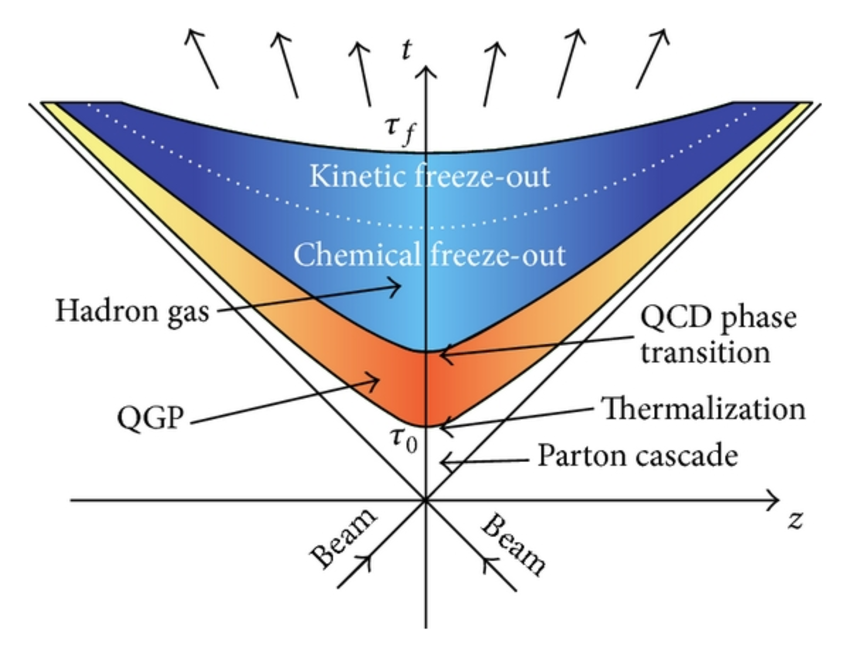
\includegraphics[width=5in]{Chapter1/importfigs/The-space-time-evolution-of-heavy-ion-collision-The-figure-is-taken-from-28.png}
\par\end{centering}
\caption{History of a Heavy-Ion Collision \cite{Wang:2012jua}\label{fig:historyHI}}
\end{figure}

Lastly, hadronic jets would interact strongly with the QGP; therefore, dijets will have significant energy imbalance depending on the multiple interactions of the components jet with the QGP. All of these cases require a good understanding the heavy-ion initial state as a basis for comparison \cite{Vogt:1998kna}. 

The Large Hadron Collider (LHC) stands at the forefront of high energy nuclear physics research. The LHC is capable of reaching heavy-ion collision energies of up to 7 TeV per nucleon-nucleon \cite{Roland:2014jsa}\cite{Frankfurt:2005mc}\cite{Vogt:2002ve}.

\section{Wigner distribution}

The Wigner distribution was first developed as part of an attempt by Eugene Wigner to map solutions to Schrodinger equation into phase probability distributions, i.e. a statistical mechanics interpretation of quantum mechanics.
\begin{equation}
\displaystyle P(x,p)~{\stackrel {\mathrm {def} }{=}}~{\frac {1}{\pi \hbar }}\int _{-\infty }^{\infty }\psi ^{*}(x+y)\psi (x-y)e^{2ipy/\hbar }\,dy\
\end{equation}
The Wigner distribution $P(x,p)$ can be used to calculate the expectation value of any given variable by considering the Wigner tranformation $g(x,p)$ of that variable's operator, $\hat{G}$,
\begin{equation}
\displaystyle \langle {\hat {G}}\rangle =\int \!dx\,dp~P(x,p)~g(x,p)~.
\end{equation}
Notice that in order to derive expectation values, the probability distribution most be integrated with respect to a function of position or momentum, which are still non-commuting according to the uncertainty principle. 

The Wigner distribution is a quantum phase space distribution that describes elliptic gluons \cite{Belitsky:2003nz}. Specifically, by considering the color diple scattering amplitude, the angular correlation of the nucleon recoil momentum and the dijet transverse momentum can provide a three-dimensional, tomographic image of the gluons within a high energy nucleus. This tomographic image takes the form of a Wigner distribution, which contains all the information of both TMDs and GPDs without violating the uncertainty principle. Specifically, the angular correlation directly measures the Fourier transform of the gluons. This is possible because the dipole amplitudes are functions of the impact parameter, and because collinear factorization holds. 

\begin{figure}[h!]
\begin{centering}
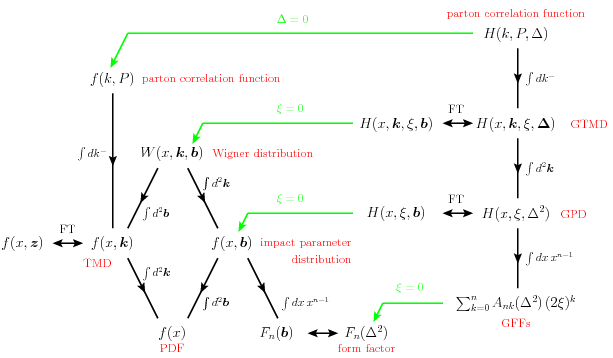
\includegraphics[width=7in]{Chapter1/importfigs/fig6_introGPD_TMD.png}
\par\end{centering}
\caption{Interconnectedness of Parton Distributions \cite{Diehl:2003ny} \label{fig:gpdTMDWeb}}
\end{figure}

TMDs and GPDs manifest non-perturbative QCD effects. The Wigner distribution, at this scale, reflects the relationship between the position and momentum of partons. Integrating the Wigner function over the transverse distance yields the TMD, while integrating over transverse momentum yields a GPD with spatial information. 

Yoshitaka Hatta uses the dipole framework to show that the azimuthal angular correlations of coherent dijets are generated by the underlying Wigner distribution of the small-x gluons. Furthermore, these correlations are consistent with predictions based on standard collinear factorization. Relevant kinematic variables are mapped in the figure \ref{fig:yatta1}. The diagram shows a virtual photon interacting with a nucleon. $k_1$ and $k_2$ are the transverse momenta of the final state jets. These jets originate from a quark-antiquark pair. 

\begin{figure}[h!]
\begin{centering}
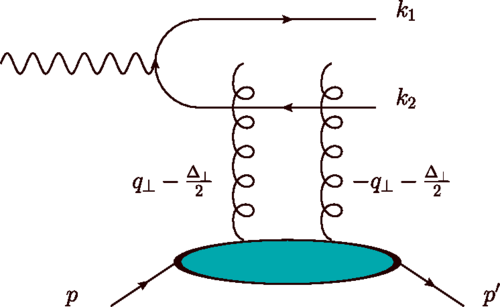
\includegraphics[width=4in]{Chapter1/importfigs/fig4_yatta.png}
\par\end{centering}
\caption{Feynman Diagram of Coherent Dijets in Dipole Framework \cite{Hatta:2016dxp}\label{fig:yatta1}}.
\end{figure}

It is expected that the dominant contribution to the angular correlation is the ellipitic, corresponding to $n=2$ in the Fourier transform \cite{Ollitrault:1992bk}. The interior of the proton displays an intricate structure. UPC collisions allow an unprecedented access to the nuclear structure in general and the small-x gluons in particular \cite{Altinoluk:2015dpi}. Figure \ref{fig:sixPlot} shows the theoretical calculation of the elliptic quark distribution - GTMD - for the $u$ and $d$ quarks; notice that for small-x values and large proton recoil, the $GTMD$ is enhanced \cite{Chakrabarti:2016yuw}. 

\begin{figure}[htp]
  \centering
  \label{fig:sixPlot}\caption{Theoretical Quark GTMDs \cite{Chakrabarti:2016yuw}}
  
  \subfloat[]{\label{figur:1}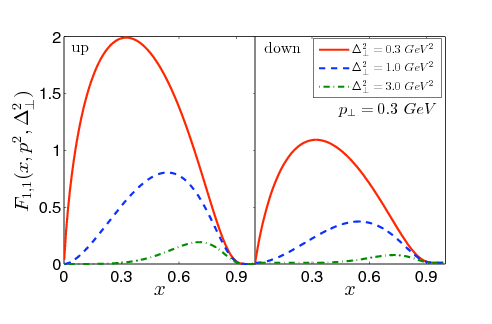
\includegraphics[width=90mm]{Chapter1/importfigs/chakraburti_1.png}}
  \subfloat[]{\label{figur:2}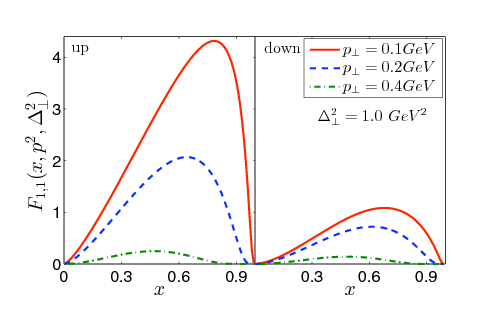
\includegraphics[width=90mm]{Chapter1/importfigs/chakraburti_2.png}}
  \\
  \subfloat[]{\label{figur:3}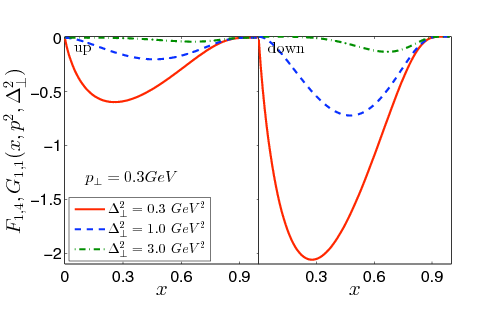
\includegraphics[width=90mm]{Chapter1/importfigs/chakraburti_3.png}}
  \subfloat[]{\label{figur:4}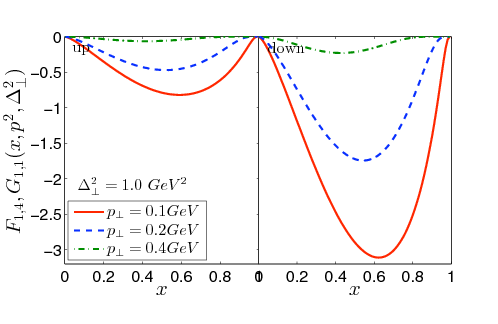
\includegraphics[width=90mm]{Chapter1/importfigs/chakraburti_4.png}}
  \\
  \subfloat[]{\label{figur:5}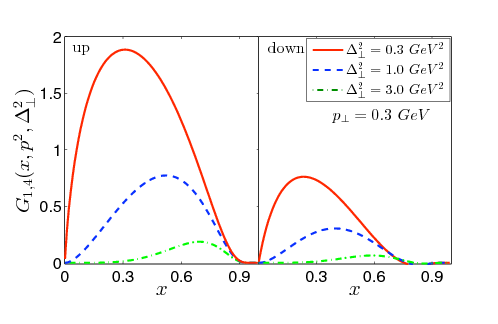
\includegraphics[width=90mm]{Chapter1/importfigs/chakraburti_5.png}}
  \subfloat[]{\label{figur:6}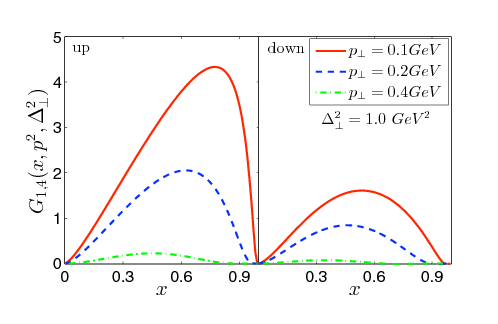
\includegraphics[width=90mm]{Chapter1/importfigs/chakraburti_6.png}}

\end{figure}